\section{Results}
To demonstrate \deploy's capability conduct transition
scenario analysis effectively and meet the objectives described in section 
\ref{sec:obj}, this section will: 
\begin{enumerate}
\item demonstrate \deploy's capabilities in a simple transition scenario, 
\item compare the use of different \deploy prediction methods in EG01-EG23, EG01-EG24, 
EG01-EG29, and EG01-EG30 transition scenarios, 
\item compare the use of varied power buffer sizes in EG01-EG23, EG01-EG24, 
EG01-EG29, and EG01-EG30 transition scenarios, and
\item demonstrate successful \deploy setup of EG01-EG23, EG01-EG24, 
EG01-EG29, and EG01-EG30 transition scenarios using the prediction method and 
power buffer size that proved best in the previous sections. 
These will be referred to as "best performance models". 
\end{enumerate}
The input files and scripts to reproduce the results and plots in this
paper are found in \cite{chee_arfc/d3ploy:_2019} and 
\cite{bae_arfctransition-scenarios_2019}. 

\subsection{Demonstration of \deploy's Capabilities}
\label{sec:demo}
We conducted a simple transition scenario simulation with
linearly increasing power demand
to demonstrate \deploy's capabilities and inform input parameter 
choices when setting up complex many-facility transition scenarios. 
This simulation is defined as \textit{simple} since 
it only includes
three facility types: \texttt{source}, \texttt{reactor}, and 
\texttt{sink}. 
The simulation begins with ten \texttt{reactor} facilities 
(\texttt{reactor1} to \texttt{reactor10}). 
These reactors have staggered cycle lengths and lifetimes to prevent 
simultaneous refueling and set up gradual decommissioning. 
\deploy is configured to deploy \texttt{new reactor} facilities
to meet the loss of power supply created by the decommissioning 
of the initial \texttt{reactor} facilities. 
Table \ref{tab:demonstrations} shows the \deploy input parameters 
for this simulation.  

    \begin{table}[]
        \caption{\deploy's input parameters for the simple transition 
        scenario with linearly increasing power demand.}
        \label{tab:demonstrations}
        \begin{tabular}{l|ll}
        \hline
                                  & \textbf{Input Parameters}          & \textbf{Simple Transition Scenario} \\ \hline
        \multirow{5}{*}{\textbf{Required}} & Demand driving commodity  & \multicolumn{1}{l}{Power}                            \\
                                  & Demand equation [MW]          &  $t<40 = 1000, t\geq 40 = 1000+250t$                                                    \\
                                  & Available facilities    &  \texttt{Source}, \texttt{Reactor}, \texttt{Sink}                                                    \\
                                  & Prediction method         &  \texttt{FFT}                                                    \\
                                  & Deployment driving method & \multicolumn{1}{l}{Installed Capacity}               \\ \hline
        \multirow{2}{*}{\textbf{Optional}} & Buffer type               & \multicolumn{1}{l}{Absolute}                         \\
                                  & Buffer size               &  Power: 2000MW, Fuel: 1000kg                                                    \\ \hline
        \end{tabular}%
        \end{table}

Figures \ref{fig:growingtransition-power}, \ref{fig:growingtransition-fuel},
and \ref{fig:growingtransition-spentfuel} demonstrate \deploy's capability 
to deploy reactors and supporting facilities to minimize undersupply 
when meeting linearly increasing power demand and subsequent secondary 
commodities demand. 
In Figure \ref{fig:growingtransition-power} there exists no time steps 
in which the supply of power falls under demand, meeting the main 
objective of \deploy. 
By using a combination of the \texttt{FFT} method for 
predicting demand and a power supply buffer of 2000MW 
(the capacity of 2 reactors), we minimized the number of 
undersupplied time steps for every commodity.

In figure \ref{fig:growingtransition-fuel},
a large-throughput source facility is initially
deployed to meet the large initial fuel demand for the commissioning 
of ten reactors. 
Deployment of a large-throughput source facility for the 
first few time steps ensures \deploy does not deploy supporting
facilities that become redundant at later times in  
the simulation.
This reflects reality in which reactor manufacturers accumulate
an appropriate amount of fuel inventory before starting 
up reactors. 

\begin{figure}[]
    \centering
    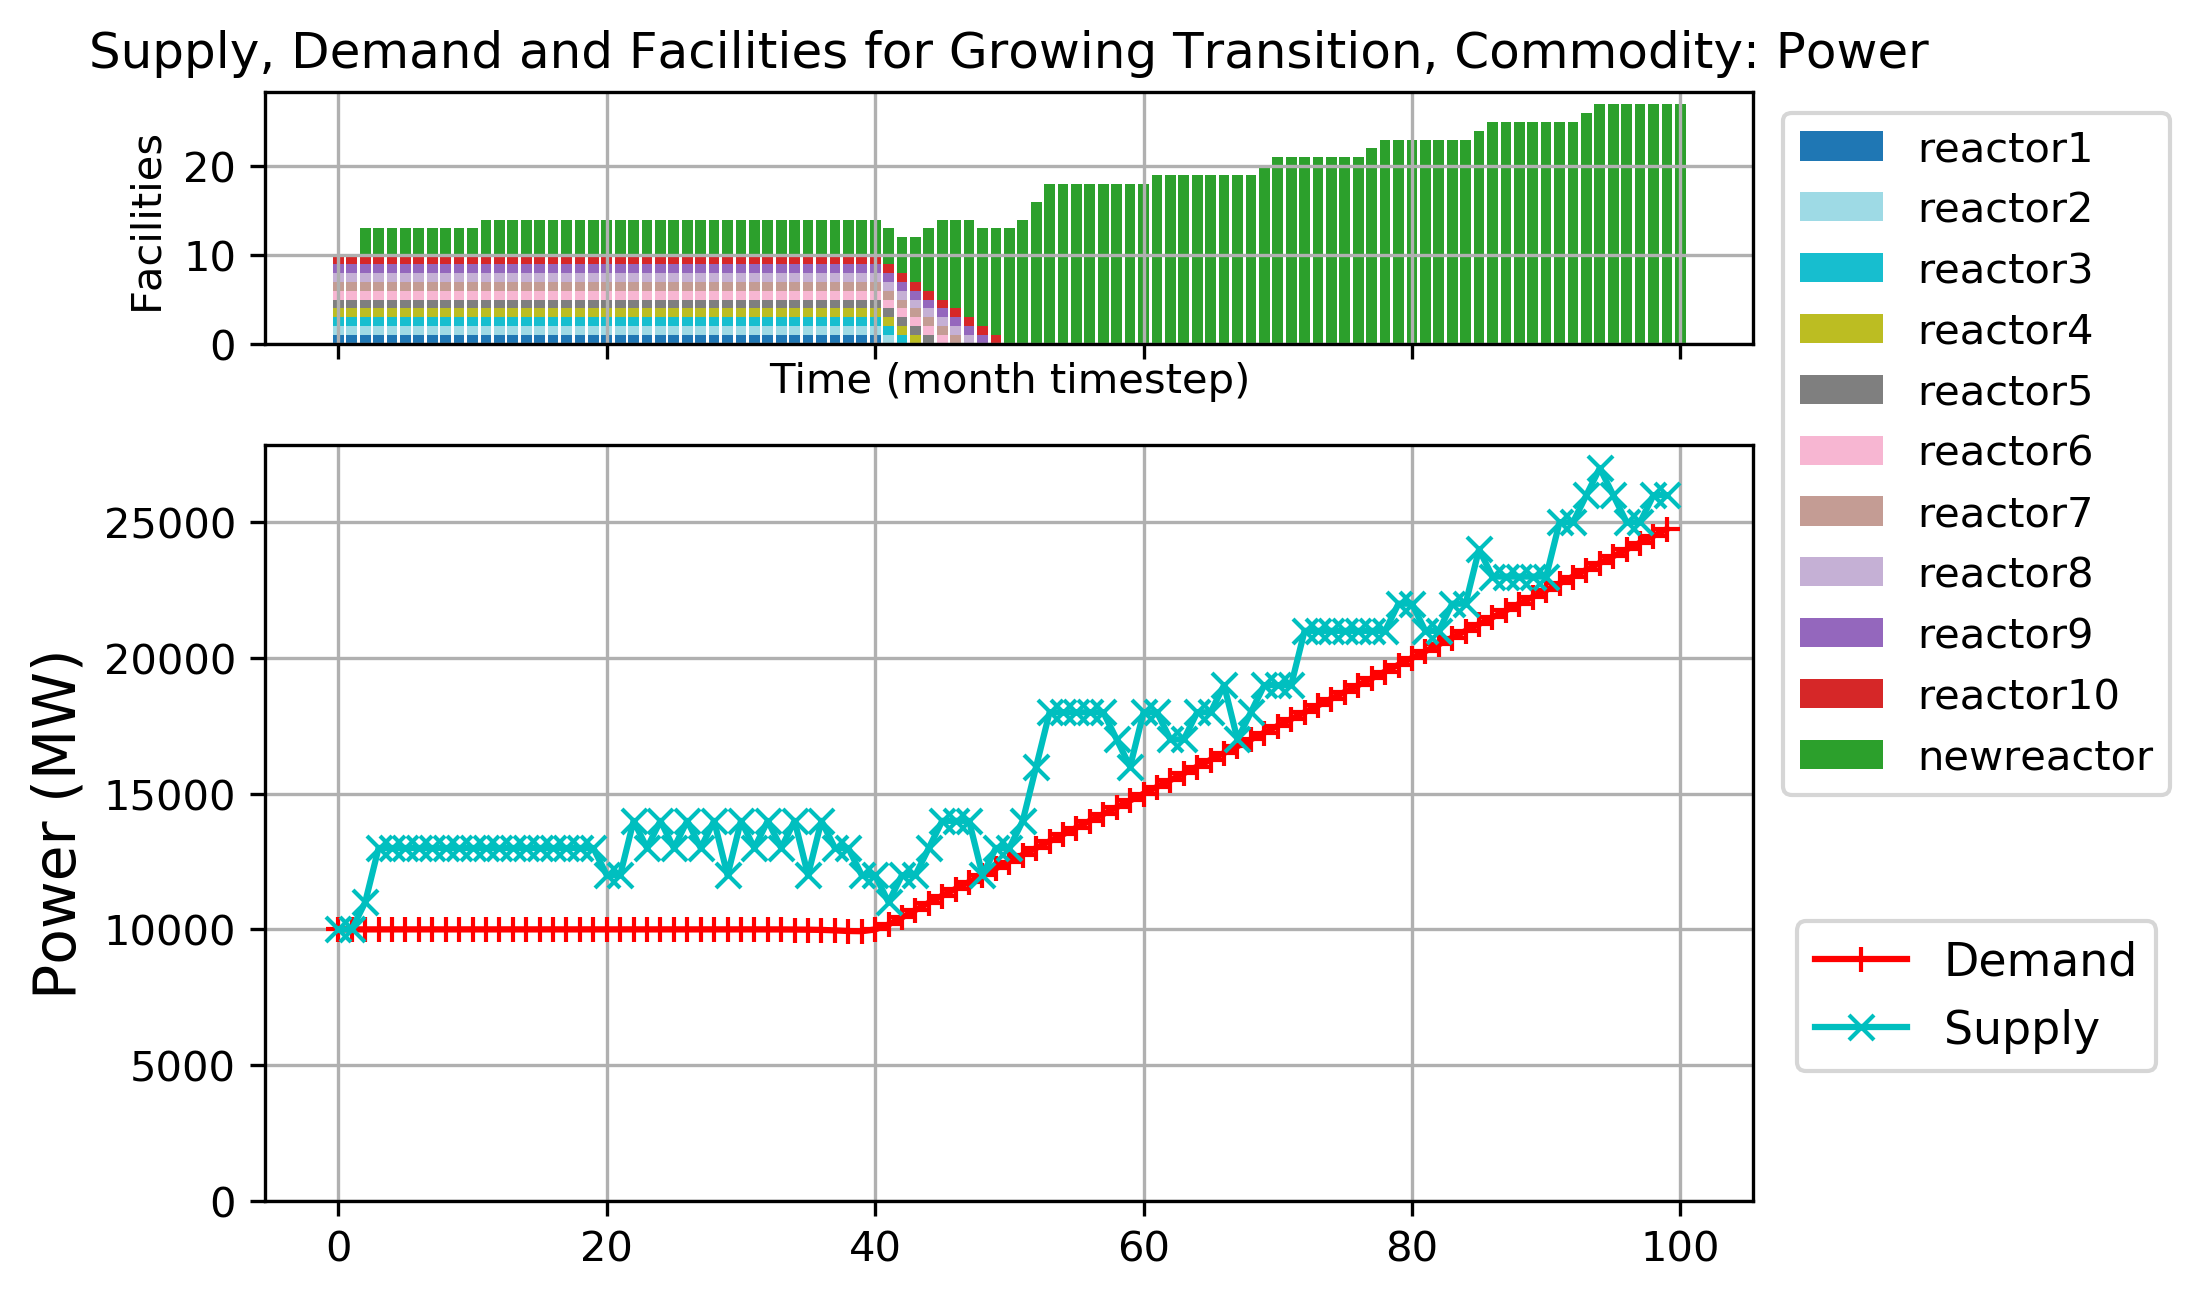
\includegraphics[width=\linewidth]{figures/growingtransition-power.png} 
        \caption{Power demand and supply, and reactor facility deployment plot for  
        a simple linearly increasing power demand transition scenario with 
        three facility types: \texttt{source}, \texttt{reactor}, and \texttt{sink}.
        The simulation begins with \texttt{reactor1} to \texttt{reactor10} and \deploy 
        deploys \texttt{newreactors} to meet increasing power demand. }
        \label{fig:growingtransition-power}
\end{figure}

\begin{figure}[]
    \centering
    \begin{subfigure}[t]{1\textwidth}
        \centering
        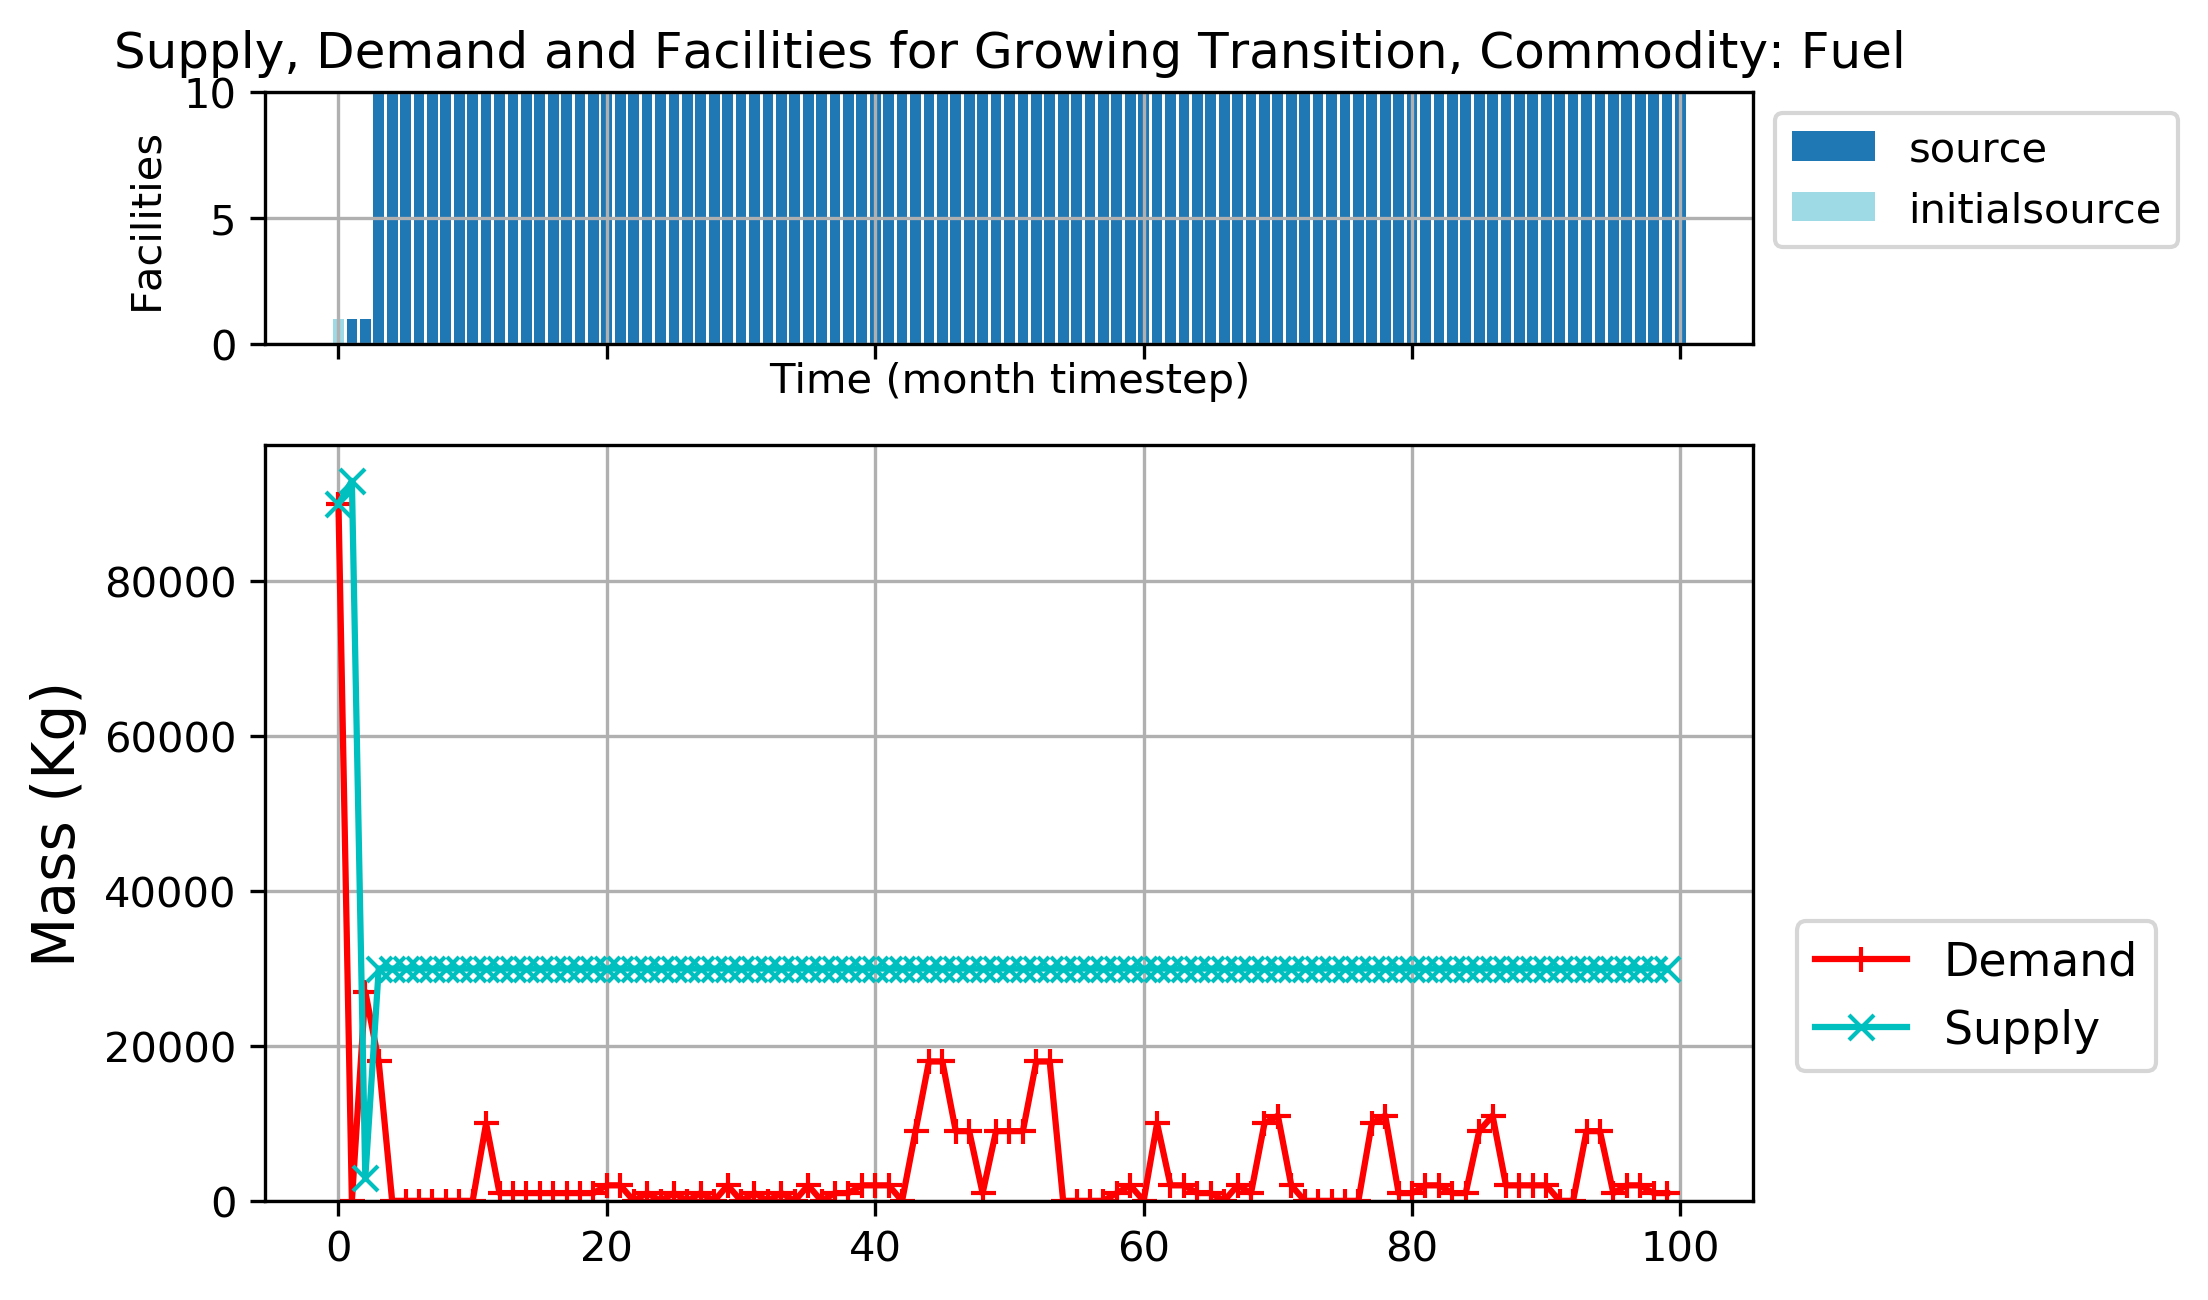
\includegraphics[width=\linewidth]{figures/growingtransition-fuel.png} 
        \caption{Fuel demand and supply, and source facility deployment plot.
        Fuel is demanded by reactors and supplied by source facilities.
        There is only one time step with undersupply of fuel.}
	    \label{fig:growingtransition-fuel}
    \end{subfigure}
    \begin{subfigure}[t]{1\textwidth}
        \centering
        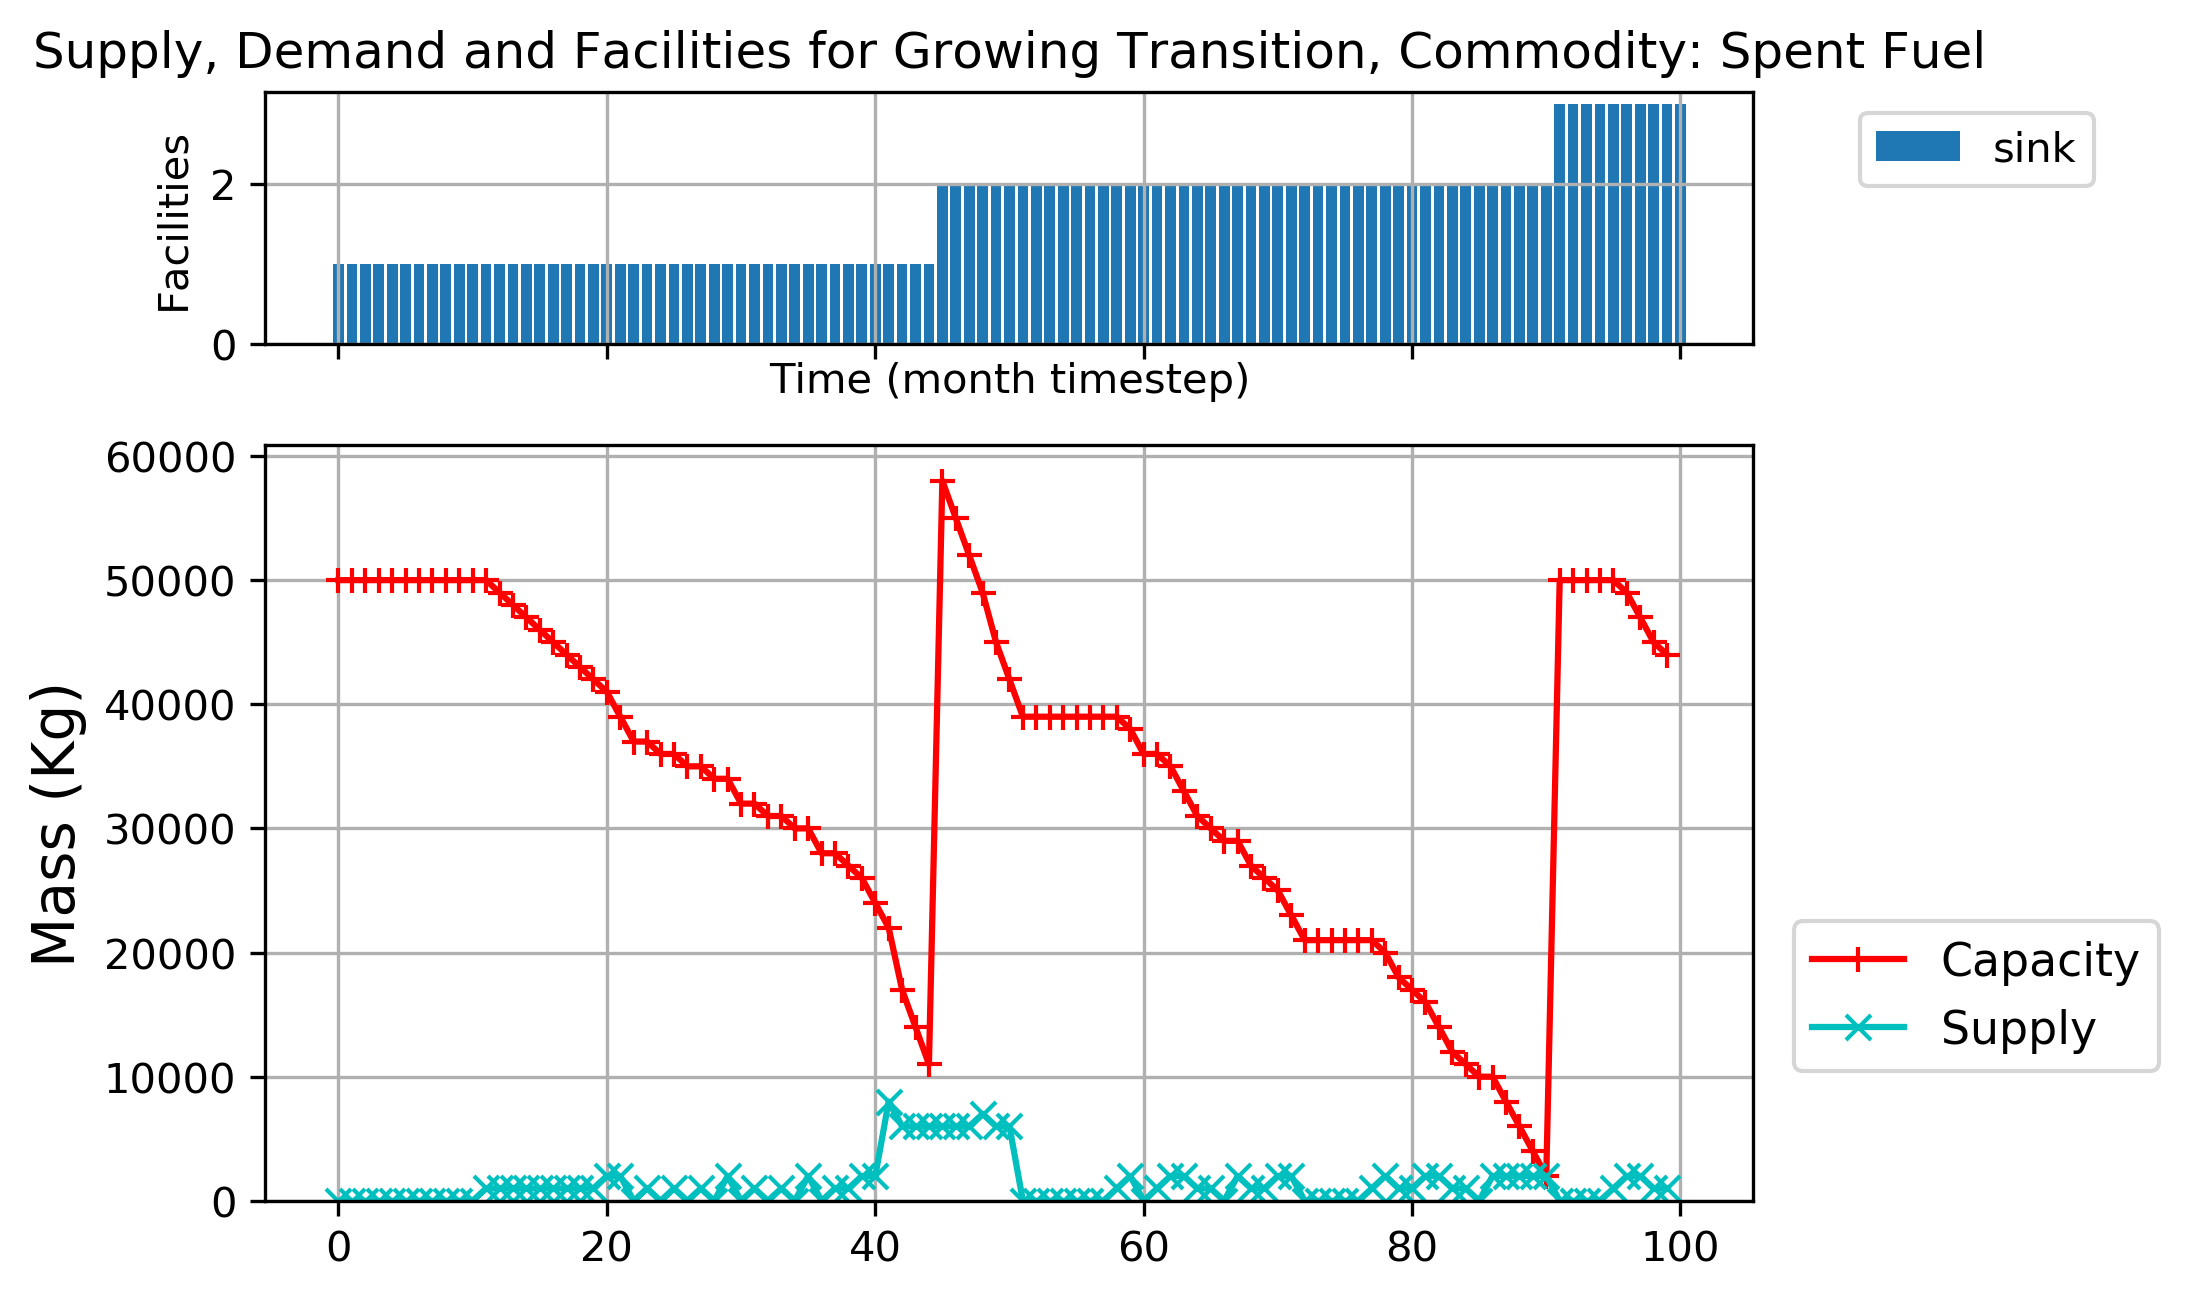
\includegraphics[width=\linewidth]{figures/growingtransition-spentfuel.png} 
        \caption{Spent fuel capacity and supply, and sink facility deployment plot.
            Spent fuel is supplied by reactors and the capacity to store them 
            is provided by sink facilities.
        There are no time steps with under-capacity of sink space.}
        \label{fig:growingtransition-spentfuel}
    \end{subfigure}
    \caption{Simple linearly increasing power demand transition scenario with 
    three facility types: \texttt{source}, \texttt{reactor}, and \texttt{sink}.}
\end{figure}
